\chapter{2023/10/30}\label{20231030}

\section{Lift 升力}\label{lift-ux5347ux529b}

\emph{Science American}: No One Can Explain Why Planes Stay in the Air
(by Ed Regis).

\emph{(Note: This article was originally published with the title ``The
Enigma of Aerodynamic Lift'' in Scientific American 322, 2, 44-51
(February 2020))}

\begin{quote}
作业:Einstein 如何解释河流的弯曲?
\end{quote}

\begin{quote}
作业:Einstein 的茶叶悖论是什么
\end{quote}

\section{Scalar triple product
标量三重积}\label{scalar-triple-product-ux6807ux91cfux4e09ux91cdux79ef}

\(\boldsymbol a, \boldsymbol b, \boldsymbol c\) can form a parallelepiped (可以组成平行六面体), as shown in Fig 13.1.

\begin{center}
    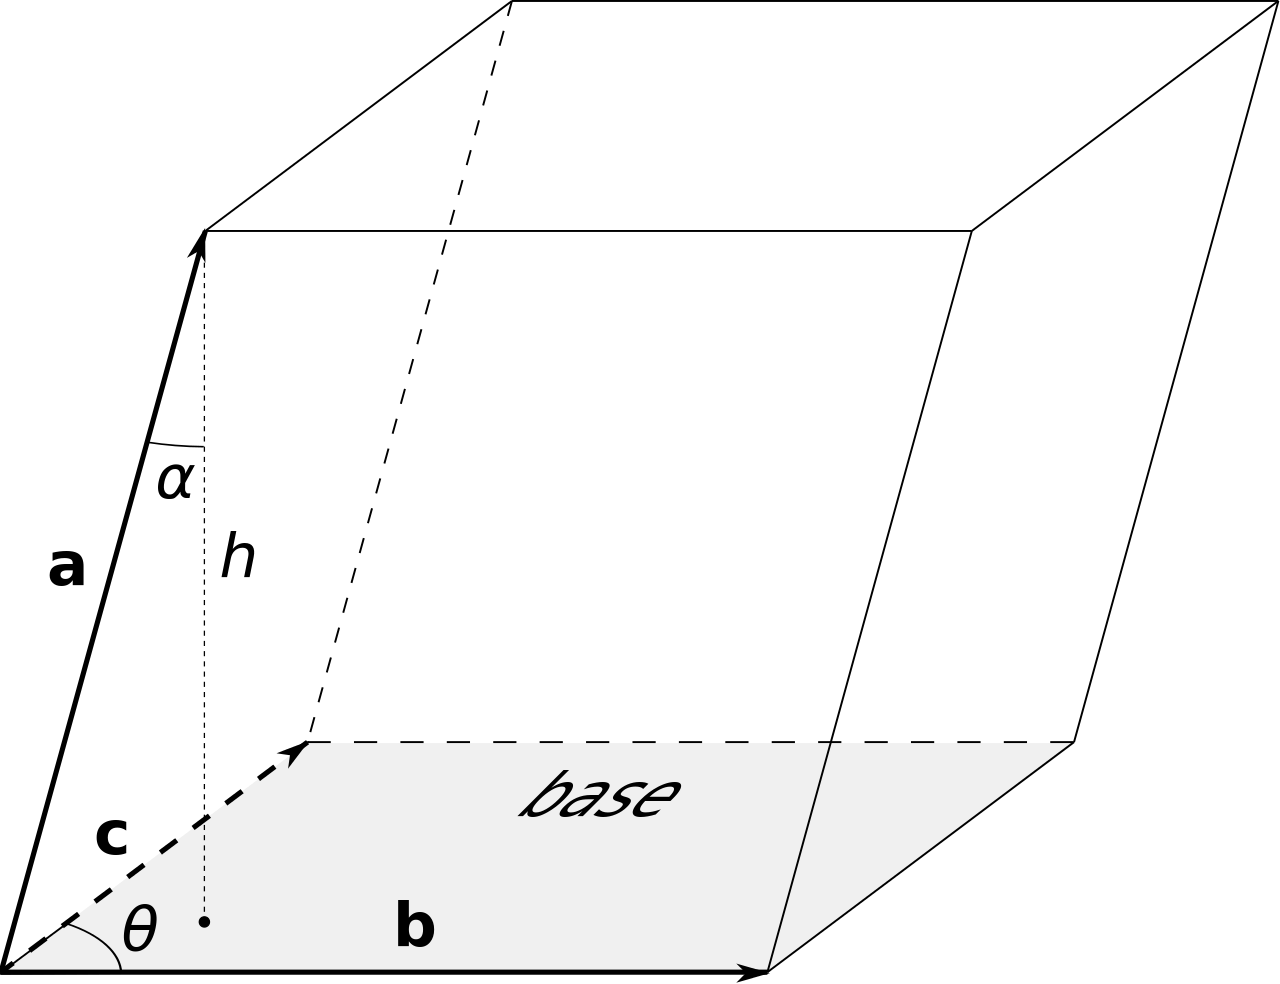
\includegraphics[height=120pt]{assets/Scalar_triple_product.png}
    \captionof{figure}{Scalar triple product}
\end{center}

The volume of this parallelepiped is
\[V = \boldsymbol a \cdot (\boldsymbol b \times \boldsymbol c) = \boldsymbol c \cdot (\boldsymbol a \times \boldsymbol b) = \boldsymbol b \cdot (\boldsymbol c \times \boldsymbol a).\]

Here,
\[\boldsymbol a \cdot (\boldsymbol b \times \boldsymbol c) = \boldsymbol a \cdot (b_i c_j \varepsilon_{ijk} \boldsymbol e_k) = b_i c_j a_k \varepsilon_{ijk},\]
\[\boldsymbol b \cdot (\boldsymbol c \times \boldsymbol a) = \boldsymbol b \cdot (c_i a_j \varepsilon_{ijk} \boldsymbol e_k) = c_i a_j b_k \varepsilon_{ijk},\]
\[\boldsymbol c \cdot (\boldsymbol a \times \boldsymbol b) = \boldsymbol c \cdot (a_i b_j \varepsilon_{ijk} \boldsymbol e_k) = a_i b_j c_k \varepsilon_{ijk},\]
where \(i\), \(j\) and \(k\) are all dumb indices (哑标).

We usually record \begin{align*}
    \begin{bmatrix} \boldsymbol a & \boldsymbol b & \boldsymbol c \end{bmatrix} & = \boldsymbol a \cdot (\boldsymbol b \times \boldsymbol c) = \boldsymbol c \cdot (\boldsymbol a \times \boldsymbol b) = \boldsymbol b \cdot (\boldsymbol c \times \boldsymbol a) \\
    & = \begin{vmatrix}
            a_1 & a_2 & a_3 \\
            b_1 & b_2 & b_3 \\
            c_1 & c_2 & c_3
    \end{vmatrix}.
\end{align*}

\section[Static equilibrium conditions 静力平衡条件]{Static equilibrium conditions (derived using virtual work)
(用虚功原理推导的)
静力平衡条件}\label{static-equilibrium-conditions-derived-using-virtual-work-ux7528ux865aux529fux539fux7406ux63a8ux5bfcux7684-ux9759ux529bux5e73ux8861ux6761ux4ef6}

In mechanics, there are two kinds of displacements (位移):

\begin{itemize}
\tightlist{}
\item real displacement 实位移
\item virtual displacement 虚位移
\end{itemize}

The static equilibrium conditions are:

\begin{itemize}
\tightlist{}
\item Resultant force 合力
    \[\sum_i \boldsymbol F_i = \boldsymbol 0\]
\item
    Resultant torque/moment 合力矩
    \[\sum_i \boldsymbol r_i \times \boldsymbol F_i = \sum_i \boldsymbol \tau_i = \boldsymbol 0\]
\end{itemize}

For a rigid body (刚体), there are 2 kinds of motion:

\begin{itemize}
\tightlist{}
\item translation 平动
\item rotation 转动
\end{itemize}

When calculating virtual work, we assume that we have 

\begin{itemize}
\tightlist{}
\item In translation: virtual displacement \(\delta \boldsymbol u_0\)
\item In rotation: virtual rotational angle \(\delta \boldsymbol \Theta\)
\end{itemize}

The resultant virtual displacement (总虚位移) is
\[\delta \boldsymbol u_i = \delta \boldsymbol u_0 + \delta \boldsymbol \Theta \times \boldsymbol r_i.\]

Virtual work is \begin{align*}
    \delta W & = \sum_i \boldsymbol F_i \cdot \delta \boldsymbol u_i \\
    & = \sum_i \left( \boldsymbol F_i \cdot \delta \boldsymbol u_0 \right) + \sum_i \left[ \boldsymbol F_i \cdot \left (\delta \boldsymbol \Theta \times \boldsymbol r_i \right) \right] \\
    & = \delta \boldsymbol u_0 \cdot \sum_i \boldsymbol F_i + \sum_i \left[ \delta \boldsymbol \Theta \cdot \left (\boldsymbol r_i \times \boldsymbol F_i \right) \right] \\
    & = \delta \boldsymbol u_0 \cdot \sum_i \boldsymbol F_i + \delta \boldsymbol \Theta \cdot \sum_i \left (\boldsymbol r_i \times \boldsymbol F_i \right).
\end{align*}

Because \(\delta \boldsymbol u_0\) and \(\delta \boldsymbol \Theta\) are
arbitrary (任意的,任取的), and work is positive definite
(功具有正定性), in equilibrium we have
\[\delta W = 0 \Rightarrow \left\{
    \begin{array}{ll}
        \delta \boldsymbol u_0 \cdot \sum_i \boldsymbol F_i = 0 & \Rightarrow  \sum_i \boldsymbol F_i = \boldsymbol 0
        \\[1.5ex]
        \delta \boldsymbol \Theta \cdot \sum_i \left (\boldsymbol r_i \times \boldsymbol F_i \right) = 0 & \Rightarrow  \sum_i \left (\boldsymbol r_i \times \boldsymbol F_i \right) = \boldsymbol 0.
    \end{array}
\right.\]
